\documentclass[10pt,a4paper]{article}
\usepackage[margin=2cm]{geometry}
\usepackage[T1]{fontenc}
\usepackage{lmodern,microtype}
\usepackage{amsmath,amssymb}
\usepackage{booktabs,tabularx,multirow}
\usepackage{graphicx}
\usepackage[font=small,labelfont=bf,skip=3pt]{caption}
\usepackage{natbib}
\usepackage[colorlinks=true,linkcolor=black,citecolor=black,urlcolor=blue]{hyperref}
\usepackage{enumitem}
\usepackage{url}
\setlist{nosep,leftmargin=1.2em}
\setlength{\parskip}{2pt}
\setlength{\abovedisplayskip}{3pt}\setlength{\belowdisplayskip}{3pt}
\newcommand{\bps}{\,\text{bps}}

\title{\vspace{-1.2cm}\textbf{Does Optimal Multivariate Pair Trading Survive DEX Frictions?}\\[2pt]
\large Extending the OTT to stablecoin arbitrage on Uniswap V3}
\author{Omar Hanabal \and Hanaa Alaoui Aboubarakate \and Sara Chraibi Houssaini \and Esteban Baptista Alves}
\date{\vspace{-0.3cm}\small Algorithmic Trading --- Group project --- November 2026}

\begin{document}
\maketitle
\vspace{-0.4cm}
\begin{abstract}\noindent
We re-implement the Optimal Trading Technique (OTT) of \citet{yang2024} and transpose it from fiat currencies on a centralised exchange to \emph{stablecoins on Uniswap V3}: ETH is priced in USDC, USDT and DAI in three on-chain pools, and the strategy trades the cross-rates implied through ETH. We extend the pipeline with (i) Johansen and Ornstein--Uhlenbeck (OU) econometrics, (ii) Kalman-filter state-space trading bands, (iii) a mean--CVaR allocation with a convex price-impact term and a friction-aware entry rule, and (iv) explicit pool fee tiers, constant-product slippage and stochastic gas. On 15-minute CoinGecko on-chain data (May--Nov 2026, walk-forward, out-of-sample), the paper's rule loses \$46.4k with its flat 0.1\% fee and \$1.4k with real DEX frictions. The friction-aware variants are profitable on 94--100\% of trades, but the edge is tiny (+\$92 to +\$177 on \$750k): cross-pool mispricings close within one 15-minute bar and capacity is limited by pool depth.
\end{abstract}

\section{Asset selection and research design}
OTT forms a ``bucket'' of quote currencies for one liquid anchor asset (ETH) and arbitrages the temporary de-synchronisation of the ETH price across quotes, without ever holding ETH. On Ethereum the same structure exists natively: ETH trades against USDC, USDT and DAI in \emph{separate} Uniswap V3 pools, with their own liquidity providers, order flow and fee tiers. With $P_{c,t}$ the price of one ETH in stablecoin $c$, the ratio $P_{\text{USDT},t}/P_{\text{USDC},t}$ is the USDC/USDT exchange rate implied through ETH. Its deviations from equilibrium have two sources: \emph{peg risk} (issuers, collateral and redemption channels differ) and \emph{pool microstructure} (one-sided swaps move one pool before arbitrage bots realign the others). Both are mean-reverting while pegs hold, which is the property pair trading needs, and the fat-tailed de-peg risk motivates a tail-risk measure (CVaR) instead of variance.

Our design differs from the paper on every forbidden dimension: venue and data (Uniswap V3 on-chain swaps via the CoinGecko API instead of Kraken), assets (stablecoins instead of USD/CAD/GBP/EUR), costs (pool-specific fees, slippage, gas instead of a flat 0.1\%), frequency (15 minutes, with 4 hours as robustness check; the paper used 1/5/60 minutes) and period (May--Nov 2026). We use the deepest fee tier of each pair, 0.05\% (pools \texttt{0x88e6\ldots5640}, \texttt{0x11b8\ldots97f6}, \texttt{0x6059\ldots a270}).

\section{Data}
\textbf{Prices.} 15-minute OHLCV candles of each pool are downloaded from the CoinGecko on-chain API (endpoint \path{/onchain/networks/eth/pools/{pool}/ohlcv/minute}, \texttt{aggregate=15}), quoted as the price of WETH \emph{in the pool's stablecoin} (\texttt{currency=token}), which preserves de-peg information that a USD price would erase. The window is 20 May 14:30 -- 14 Nov 2026 14:15 UTC (17{,}088 bars; the free tier serves six months). Pools are aligned on one grid; bars without a swap are forward-filled for at most 30 minutes; the candle still forming at download time is discarded. Figure~\ref{fig:spreads} shows the implied cross-rates: USDT trades at a mean premium of $+6.6\bps$ (s.d.\ $8.1\bps$) relative to USDC through ETH; the DAI pool, whose liquidity has migrated to USDS, is much noisier (s.d.\ $26\bps$, with isolated bad prints).

\textbf{Gas and depth.} The EIP-1559 base fee plus median priority fee is read from a public Ethereum node with \texttt{eth\_feeHistory} at every hourly close (4{,}273 samples) and forward-filled to 15 minutes; it lies mostly between 0.1 and 1 gwei, i.e.\ below \$0.10 per swap, with spikes to \$2.5. Pool depth is the stablecoin-side \emph{virtual} reserve of the active Uniswap V3 range, $x_v=L/\sqrt{P}$ (or $L\sqrt{P}$), computed from \texttt{liquidity()} and \texttt{slot0()}: \$180M (USDC), \$45M (USDT) and \$0.6M (DAI).

\begin{figure}[t]
\centering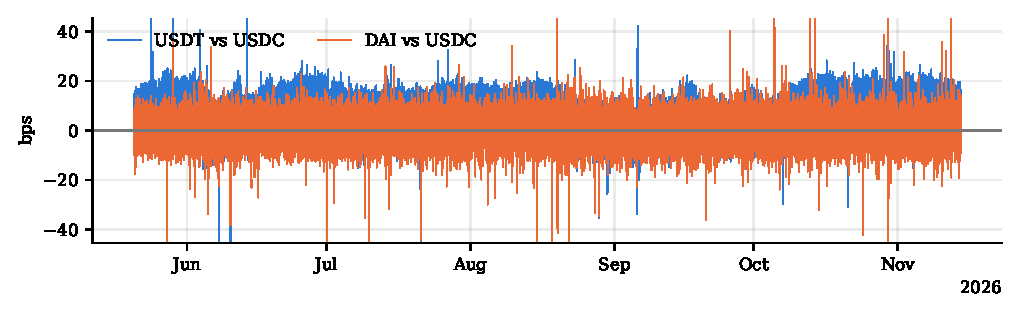
\includegraphics[width=\linewidth]{figures/fig_spreads.pdf}
\vspace{-14pt}\caption{Relative price of ETH in USDT and DAI versus USDC, $P_{c,t}/P_{\text{USDC},t}-1$ (bps, 15-min closes, y-axis clipped at the 99.9th percentile).}\label{fig:spreads}
\vspace{-6pt}
\end{figure}

\section{Methodology}
\textbf{Spread and screening.} For a pair $(i,j)$ the spread is $s_{ij,t}=\ln P_{i,t}-\ln P_{j,t}$, i.e.\ the log cross-rate, so the hedge ratio is 1 by construction. As in the paper, a pair is kept if the average weekly Pearson correlation exceeds 0.9 and the Engle--Granger test rejects non-cointegration in at least 30\% of weekly windows. \emph{Extension 1a:} the Johansen trace test is applied to the whole bucket through the VECM $\Delta\mathbf{p}_t=\alpha\beta^\top\mathbf{p}_{t-1}+\Gamma_1\Delta\mathbf{p}_{t-1}+\varepsilon_t$; with $n$ quotes of one common stochastic trend, theory predicts rank $r=n-1$.

\textbf{Ornstein--Uhlenbeck spread (Extension 1b).} We model $ds_t=\theta(\mu-s_t)dt+\sigma dW_t$, whose exact discretisation on step $\Delta$ is the AR(1) $s_{t+1}=a+bs_t+\varepsilon_t$ with $b=e^{-\theta\Delta}$, $\mu=a/(1-b)$, $\sigma_{eq}=\sigma_\varepsilon/\sqrt{1-b^2}$ and half-life $t_{1/2}=\ln 2/\theta$, estimated by OLS on the formation window. It replaces the paper's ad-hoc ``average reversion time'' $mr$: the expected reversion of a deviation over a horizon $h$ is $\mathbb{E}[s_t-s_{t+h}]=(s_t-\mu)(1-e^{-\theta h})$, and the OU forecast errors $e_k=(s_{k+h}-s_k)-(\mu-s_k)(1-e^{-\theta h})$ provide the risk scenarios.

\textbf{State-space signals (Extension 2).} The paper's static $z_t=(s_t-\bar s)/\hat\sigma_s$ keeps firing when the fair cross-rate shifts. We write $s_t=m_t+x_t$, with a slow random-walk fair value $m_t=m_{t-1}+\eta_t$ and an AR(1) deviation $x_t=\phi x_{t-1}+\nu_t$, estimate $(\sigma^2_\eta,\sigma^2_\nu,\phi)$ by maximum likelihood on formation data only (capping $\sigma^2_\eta\le 2\%\operatorname{Var}(x)$), and run the Kalman filter causally. The band is centred on $\hat m_{t|t}$ with width $\sqrt{\operatorname{Var}(x)+P^m_{t|t}}$, so it widens when the filter is uncertain about the fair value: $z_t=(s_t-\hat m_{t|t})/\sqrt{\sigma^2_\nu/(1-\phi^2)+P^m_{t|t}}$. Positions open when $|z_t|>z_{open}$ and close when $|z_t|<z_{close}$, when $z$ changes sign, when $|z|>6$ (stop-loss) or after six half-lives.

\textbf{Market frictions.} A spread trade is four swaps (buy ETH with $j$, sell it for $i$; reverse at closing), so the book never holds ETH and the paper's market-neutrality constraint holds by construction. Each swap pays the pool's fee tier $f_c$ on the input, slippage on the constant-product curve of the virtual reserves, $\text{out}=R_{out}\,a(1-f)/(R_{in}+a(1-f))$, and gas $G\cdot(\text{baseFee}_t+\text{tip}_t)\cdot10^{-9}\cdot P^{ETH}_t$ with $G=150{,}000$.

\textbf{Mean--CVaR allocation (Extension 3).} When signals coincide, the weight $w_n\in[0,0.5]$ of NAV for each signalled pair solves
\begin{equation*}
\max_{w}\ \sum_n w_n EP_n-\sum_n\kappa_n w_n^2-\lambda\,\mathrm{CVaR}_{95\%}\Big(-\sum_n w_n r_{\cdot,n}\Big)
\ \text{ s.t. }\ \sum_{n\,\text{spends}\,c}w_n\le\mathrm{avail}_c,\ \ \sum_n w_n\le1,
\end{equation*}
where $EP_n=|s_n-\hat m_n|(1-e^{-\theta_n h})-2(f_i+f_j)$ is the OU expected net return ($h=3$ half-lives), $\kappa_n=2\,\mathrm{NAV}(1/D_i+1/D_j)$ is the convex price-impact cost implied by the pool depths, the capital constraint is the paper's eq.~(4), and the scenarios $r_{k,n}=EP_n-d_n e_{k,n}$ are joint (same dates for all pairs). CVaR is linearised as in \citet{rockafellar2000}. Unlike variance, CVaR is in return units, so $\lambda$ keeps its meaning when spreads are measured in bps (with the paper's $\lambda=1$, $w^\top\Sigma w\approx10^{-8}$ is negligible). Because $\mathrm{CVaR}(w r)=w\,\mathrm{CVaR}(r)$ for $w\ge0$, a single signal has the closed form $w^\ast=\min\{(EP-\lambda\,\mathrm{CVaR}(r))^+/(2\kappa),\,\mathrm{cap}\}$, verified against the convex solver. Finally, a trade is executed only if its expected profit exceeds fees, slippage and four gas payments (\emph{friction-aware entry}).

\section{Backtest design}
The paper selects its thresholds by a grid search over a period overlapping its test period. We use a rolling walk-forward instead: on each 30-day formation window we re-estimate screening, Johansen, OU, the Kalman model, the scenarios and $(z_{open},z_{close})\in\{2,2.5,3\}\times\{0,0.5\}$ (best formation Sharpe), then trade the next 10 days with frozen parameters (15 blocks; out-of-sample period 19 Jun -- 14 Nov 2026, 14{,}208 bars). Signals are computed on bar closes and executed at the next bar's open. The capital is \$250k in each stablecoin; P\&L is measured in USDC. Because USDT and DAI balances are marked through ETH-implied rates, we also report the \emph{active} P\&L, net of a passive hold of the initial basket, which isolates the arbitrage. Five variants isolate each contribution: \textbf{A} paper replica (static bands, mean--variance, flat 0.1\% fee, no slippage/gas, no filter); \textbf{B} = A with DEX frictions; \textbf{C} = B + entry filter + CVaR; \textbf{D} = C with Kalman bands (full model); \textbf{E} = D with variance instead of CVaR. Fifteen automated tests (causality of every signal, market neutrality under ETH price scaling, closed form vs.\ solver, OU and Johansen recovery) are in the repository.

\section{Results}
\textbf{Econometrics.} All three pairs pass screening in every block; the Johansen rank is 2 in 9 blocks and 3 in 6. A rank of 3 would mean ETH itself is stationary; in simulations with one common trend we find that the last trace test over-rejects (20--40\% instead of 5\%), so we read it as ``all spreads stationary''. The OU half-life hits its floor of one bar in every block: the lag-1 autocorrelation of the spread is 0.32 for USDC:USDT (half-life $\approx9$ minutes) and $\approx0$ for the DAI pairs. \emph{Mispricings close within one 15-minute bar}, and within one 4-hour bar in the robustness run.

\begin{table}[t]
\centering\small
\caption{Out-of-sample performance, 15-min bars, 19 Jun -- 14 Nov 2026. Sharpe is annualised with $r_f=4\%$; ``active'' is net of the passive stablecoin basket ($r_f=0$). Win/loss = \#wins/\#losses as in the paper. P\&L is the sum of closed-trade P\&L net of all costs.}\label{tab:main}
\setlength{\tabcolsep}{3.5pt}
\begin{tabular}{@{}lrrrrrrrrr@{}}
\toprule
 & Ann.\ ret. & Sharpe & Max DD & Active ret. & Active SR & Trades & \% win & Win/loss & P\&L (\$)\\
\midrule
A\ \ Paper replica (0.1\% fee) & $-14.73\%$ & $-1.71$ & $-7.53\%$ & $-14.55\%$ & $-6.89$ & 142 & 13.4 & 0.15 & $-46{,}389$\\
B\ \ + DEX frictions & $-0.67\%$ & $-0.36$ & $-2.02\%$ & $-0.47\%$ & $-2.75$ & 176 & 15.3 & 0.18 & $-1{,}446$\\
C\ \ + entry filter, CVaR & $-0.14\%$ & $-0.31$ & $-1.83\%$ & $+0.058\%$ & $2.11$ & 17 & 94.1 & 16.0 & $+177$\\
D\ \ + Kalman (full model) & $-0.17\%$ & $-0.32$ & $-1.84\%$ & $+0.030\%$ & $1.69$ & 14 & 100 & $\infty$ & $+92$\\
E\ \ full, variance & $-0.16\%$ & $-0.32$ & $-1.84\%$ & $+0.040\%$ & $1.79$ & 17 & 100 & $\infty$ & $+121$\\
\midrule
Hold stablecoin basket & $-0.20\%$ & $-0.32$ & $-1.84\%$ & -- & -- & -- & -- & -- & --\\
Buy \& hold ETH & $+23.5\%$ & $0.59$ & $-33.8\%$ & -- & -- & -- & -- & -- & --\\
\bottomrule
\end{tabular}
\vspace{-4pt}
\end{table}

\begin{figure}[t]
\centering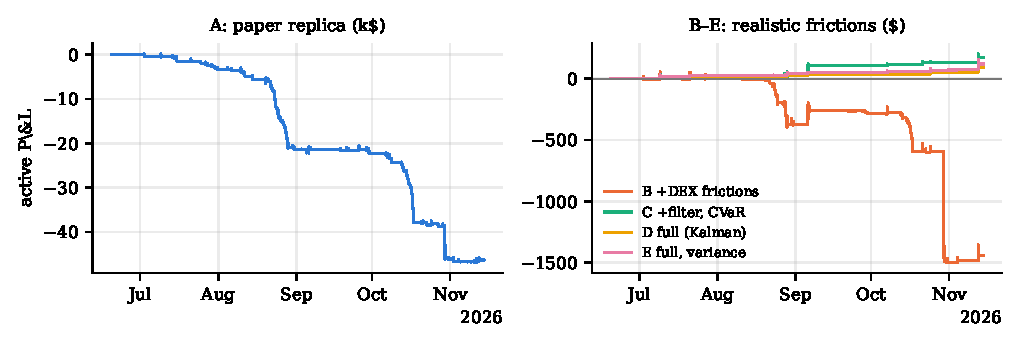
\includegraphics[width=\linewidth]{figures/fig_pnl.pdf}
\vspace{-14pt}\caption{Cumulative active P\&L (strategy minus passive stablecoin basket). Left: paper replica (k\$). Right: realistic variants (\$).}\label{fig:pnl}
\vspace{-8pt}
\end{figure}

\textbf{Performance (Table~\ref{tab:main}, Figure~\ref{fig:pnl}).} The paper's rule (A) trades 142 times, wins only 13\% of trades and loses \$46.4k, paying \$137k of fees: with mispricings closing within the bar, the signal is already stale at execution and the flat 0.1\% fee per swap dominates. Realistic DEX costs (B) are smaller because the 0.05\% tier is cheaper and the slippage term shrinks positions (USDC:USDT notional $\approx\$20$k, DAI pairs $\approx\$350$), but the rule still loses \$1.4k (fees \$2{,}253, slippage \$1{,}354, gas \$510). The \emph{friction-aware entry} is the decisive extension: it removes 90\% of the trades and turns the strategy profitable (C: 94\% winners, active Sharpe 2.1). The Kalman bands (D) and the CVaR objective (C vs.\ E) do not improve on it at this scale: every remaining trade is a single, short (0.4--0.5\,h) signal, where the closed-form CVaR and variance allocations differ only through the size of the trade. Total returns stay slightly negative because the NAV drawdown ($\approx-1.8\%$) comes from marking USDT/DAI in USDC, which is identical for the passive basket; the active drawdown is below $0.01\%$.

\textbf{Sensitivity and robustness.} Table~\ref{tab:sens} shows that the pool fee tier, not gas, is the binding friction: at 0.01\% the full model trades 216 times (99\% winners, active Sharpe 7.0, $+0.45\%$ a year), at 0.3\% it never trades. A higher $\lambda$ trades less and earns less. Absolute P\&L is almost independent of capital (\$25k to \$2.5M per coin), so the return in \% falls proportionally: capacity is set by pool depth. On 4-hour bars the paper replica also loses ($-4.3\%$ a year, 4\% winners) and the friction-aware variants trade once, confirming that coarser sampling cannot catch the mispricings.

\begin{table}[t]
\centering\footnotesize
\caption{Sensitivity of the full model D (fixed thresholds $z_{open}=2$, $z_{close}=0.5$) and 4-hour robustness run. Entries separated by ``/'' follow the order of the ``Value'' column.}\label{tab:sens}
\setlength{\tabcolsep}{4pt}
\begin{tabular}{@{}llrrrr@{}}
\toprule
Test & Value & Trades & \% win & Active ann.\ ret.\ (\%) & Active Sharpe\\
\midrule
Risk aversion $\lambda$ & 0.1 / 0.5 / 1 / 2 & 17 / 14 / 10 / 9 & 100 & .036 / .029 / .022 / .013 & 1.71 / 1.62 / 1.54 / 1.57\\
Fee tier & 0.01\% & 216 & 99.1 & .446 & 7.00\\
 & 0.05\% (base) / 0.30\% & 14 / 0 & 100 / -- & .029 / 0 & 1.62 / --\\
Capital per coin & \$25k / \$250k / \$2.5M & 14 / 14 / 8 & 100 & .291 / .029 / .003 & 1.62 / 1.62 / 1.63\\
\midrule
4-hour bars & A / B / C--E & 25 / 29 / 1 & 4 / 3 / 100 & $-4.27$ / $-0.17$ / $\approx$0 & $-5.51$ / $-3.12$ / .41--.52\\
\bottomrule
\end{tabular}
\vspace{-6pt}
\end{table}

\section{Discussion and limitations}
OTT's profitability in \citet{yang2024} relies on a frictionless flat fee and on markets where cross-quote deviations persist for hours. On Uniswap V3 in 2026, arbitrage bots close ETH/stablecoin cross-pool mispricings within minutes; a strategy observing them at 15-minute (or 4-hour) frequency mostly trades stale signals, and the paper's rule loses money. Modelling DEX frictions explicitly, and refusing trades whose expected reversion does not cover them, is what makes the multivariate arbitrage marginally profitable; refinements of the bands (Kalman) and of the risk measure (CVaR) matter little once trades are this rare. The result is honest but small: \$92--\$177 over five months on \$750k, with 14--17 trades, so the Sharpe ratios carry large estimation error.

\textbf{Limitations.} (i) Six months of data (free API) and a single regime without major de-peg; (ii) pool depth measured at one block and held constant (no archive node); (iii) execution at the next bar's open without MEV, sandwich attacks or failed transactions; (iv) gas sampled hourly; (v) Johansen rank inference is distorted in finite samples. Natural extensions are block-level data (where the mispricings actually live), the 0.01\% pools, and liquid-staking tokens (stETH, rETH), whose deviations persist for days.

\vspace{-4pt}
\begin{thebibliography}{9}\setlength{\itemsep}{0pt}\small
\bibitem[Yang and Malik(2024)]{yang2024} H.~Yang, A.~Malik (2024). Optimal market-neutral multivariate pair trading on the cryptocurrency platform. \emph{Int.\ J.\ Financial Studies} 12(3):77.
\bibitem[Rockafellar and Uryasev(2000)]{rockafellar2000} R.T.~Rockafellar, S.~Uryasev (2000). Optimization of conditional value-at-risk. \emph{J.\ of Risk} 2(3):21--41.
\bibitem[Johansen(1991)]{johansen1991} S.~Johansen (1991). Estimation and hypothesis testing of cointegration vectors in Gaussian VAR models. \emph{Econometrica} 59(6):1551--1580.
\bibitem[Engle and Granger(1987)]{engle1987} R.F.~Engle, C.W.J.~Granger (1987). Co-integration and error correction. \emph{Econometrica} 55(2):251--276.
\bibitem[Adams et al.(2021)]{adams2021} H.~Adams, N.~Zinsmeister, M.~Salem, R.~Keefer, D.~Robinson (2021). \emph{Uniswap v3 Core}. Whitepaper.
\end{thebibliography}
\end{document}
